\documentclass[a4paper]{article}
\usepackage[utf8]{inputenc}
\usepackage[russian]{babel}
\usepackage{listings}
\usepackage[a4paper,margin=1.2in]{geometry}
\usepackage{indentfirst}
\usepackage{graphicx}
\usepackage{caption}
\usepackage{float}

%\setcounter{topnumber}{2}
%\setcounter{bottomnumber}{2}
%\setcounter{totalnumber}{4}
%\renewcommand{\topfraction}{0.85}
%\renewcommand{\bottomfraction}{0.85}
%\renewcommand{\textfraction}{0.15}
%\renewcommand{\floatpagefraction}{0.8}
%\renewcommand{\textfraction}{0.1}
%\setlength{\floatsep}{5pt plus 2pt minus 2pt}
%\setlength{\textfloatsep}{5pt plus 2pt minus 2pt}
%\setlength{\intextsep}{5pt plus 2pt minus 2pt}

\begin{document}

\title{Сравнение вращаемой и сдвиговой множественных развёрток по количеству вычислений целевой функции в задачах без ограничений}
\author{}
\date{}
\maketitle

\section{Реализация алгоритма с множественными развёртками}
Алгоритм реализован на языке C++ с использованием линейных структур данных для хранения поисковой информации.
Сложность выполнения каждой итерации алгоритма $O(k)$, где $k$ --- номер итерации.

Реализация поддерживает полноценную индексную схему, $\varepsilon$-резервирование и локальную адаптацию (схема Маркина-Стронгина).
Поддержки параллельных вычислений нет.

Данная реализация не использует код системы Globalizer.

\section{Классы тестовых задач и методика проведения экспериментов}

Операционные характеристики метода с различными множественнными развёртками сторились на следующих классах задач:
функции Гришагина ($F_{GR}$), GKLS 2d Simple (gklsS2d), GKLS 2d Hard (gklsH2d), GKLS 3d Simple (gklsS3d).

Для каждого класса задач и каждого типа развёртки были предприняты попытки провести следующие эксперименты:
\begin{enumerate}
  \item решить все задачи при одинаковом для всех развёрток значении $r$ с остановкой по попаданию в окрестность известного оптимума;
  \item решить все задачи при одинаковом для всех развёрток значении $r$ с остановкой по точности;
  \item решить все задачи при минимальном допустимом для каждой конфигурации развёртки в отдельности значении параметра $r$ с остановкой по попаданию в окрестность известного оптимума;
  \item решить все задачи при минимальном допустимом для каждой конфигурации развёртки в отдельности значении параметра $r$ с остановкой по точности;
\end{enumerate}

В последних двух случаях подбор минимального значения $r$ такого, что решаются все задачи класса, осуществлялся с точностью 0.1 для каждого типа
развёртки в отдельности и для каждого значения $L$ (количество развёрток).

В связи с тем, что в представленной реализации АГП используются только линейные структуры данных, не для всех классов указанные 4 типа эспериментов были проведены. Решение некоторых задач из сложных классов требует порядка $10^6$ испытаний и занимает несколько часов на одну задачу. В этом случае подобрать минимальное значение $r$ для каждой развёртки очень затратно.

В таблицах \ref{table:exp1}, \ref{table:exp2}, \ref{table:exp3}, \ref{table:exp4} указаны эксперименты, которые были проведены. Каждый эксперимент включает в себя решение всех задач класса при $l=1,2,3$ для вращаемой развёртки и $l=1,2,3,4$ для сдвиговой.

\begin{table}
\begin{center}
\caption{Эксперименты, проведённые при минимальном значении $r$ с остановкой по попаданию в окрестность оптимума}
  \begin{tabular}{l|l*{4}{c}r}
    \label{table:exp1}
  Тип развёртки & $F_{GR}$ & gklsS2d & gklsH2d & gklsS3d \\
  \hline
  вращаемая, $L=1$ & + & + & + & + \\
  вращаемая, $L=2$ & + & + & + & + \\
  вращаемая, $L=3$ & + & + & + & + \\
  сдвиговая, $L=1$ & + & + & + & + \\
  сдвиговая, $L=2$ & + & + & + & + \\
  сдвиговая, $L=3$ & + & + & + & + \\
  сдвиговая, $L=4$ & + & + & - & - \\
  \end{tabular}
\end{center}
\end{table}

\begin{table}
\begin{center}
\caption{Эксперименты, проведённые при минимальном значении $r$ с остановкой по точности}
  \begin{tabular}{l|l*{4}{c}r}
    \label{table:exp2}
  Тип развёртки & $F_{GR}$ & gklsS2d & gklsH2d & gklsS3d \\
  \hline
  вращаемая, $L=1$ & + & + & + & - \\
  вращаемая, $L=2$ & + & + & + & - \\
  вращаемая, $L=3$ & + & + & - & - \\
  сдвиговая, $L=1$ & + & + & + & - \\
  сдвиговая, $L=2$ & + & + & - & - \\
  сдвиговая, $L=3$ & + & + & - & - \\
  сдвиговая, $L=4$ & + & + & - & - \\
  \end{tabular}
\end{center}
\end{table}

\begin{table}
\begin{center}
\caption{Эксперименты, проведённые при одинаковом значении $r$ с остановкой по попаданию в окрестность оптимума}
  \begin{tabular}{l|l*{4}{c}r}
    \label{table:exp3}
  Тип развёртки & $F_{GR}$ & gklsS2d & gklsH2d & gklsS3d \\
  \hline
  вращаемая, $L=1$ & + & + & + & + \\
  вращаемая, $L=2$ & + & + & + & + \\
  вращаемая, $L=3$ & + & + & + & + \\
  сдвиговая, $L=1$ & + & + & + & + \\
  сдвиговая, $L=2$ & + & + & + & + \\
  сдвиговая, $L=3$ & + & + & + & + \\
  сдвиговая, $L=4$ & + & + & - & - \\
  \end{tabular}
\end{center}
\end{table}

\begin{table}
\begin{center}
\caption{Эксперименты, проведённые при одинаковом значении $r$ с остановкой по точности}
  \begin{tabular}{l|l*{4}{c}r}
    \label{table:exp4}
  Тип развёртки & $F_{GR}$ & gklsS2d & gklsH2d & gklsS3d \\
  \hline
  вращаемая, $L=1$ & + & + & + & + \\
  вращаемая, $L=2$ & + & + & + & + \\
  вращаемая, $L=3$ & + & + & - & - \\
  сдвиговая, $L=1$ & + & + & + & + \\
  сдвиговая, $L=2$ & + & + & - & - \\
  сдвиговая, $L=3$ & + & + & - & - \\
  сдвиговая, $L=4$ & + & + & - & - \\
  \end{tabular}
\end{center}
\end{table}

Во всех экспериментах с остановкой по попаданию в окрестность глобального минимума использовалось значение
$\varepsilon=10^{-2}$. При остановке по точности $\varepsilon \in [10^{-3};5\cdot 10^{-3}]$ в зависимости от класса задач.
Также в некоторых случаях для ограничения, порождаемого сдвиговой развёрткой, использовалось $\varepsilon$-резервирование
величиной 0.05. Для сложных классов был задействован смешанный локально-глобальный алгоритм с параметром смешивания $q=4$.

\subsection{Опeрационные характеристики}
Операционные характеристики были построены практически для всех столбцов таблиц из предыдущего раздела.
В случае сдвиговой развёртки наличие дополнительного ограничения не учитывались при построении операционных характеристик.
При проведении экспериментов было замечено, что включение $\varepsilon$-резервирования практически не влияет на среднее
количество вычислений целевой функции и на вид операционной характеристики.

\subsubsection{Класс $F_{GR}$}
Преимущество сдвиговой развёртки над стандартным методом наблюдается только при минимальном значении $r$, причём в случае остановки по точности,
ускорение сходимости более заметно. Ускорения от использования вращаемой развёртки нет.

В случае остановки по попаданию в окрестность, сдвиговая развёртка теряет преимущество, но наблюдается интересный эффект
ускорения от её использования при $L=1$, когда метод работает с одной развёрткой и "нулевым" ограничением.

\begin{figure}
  \center
  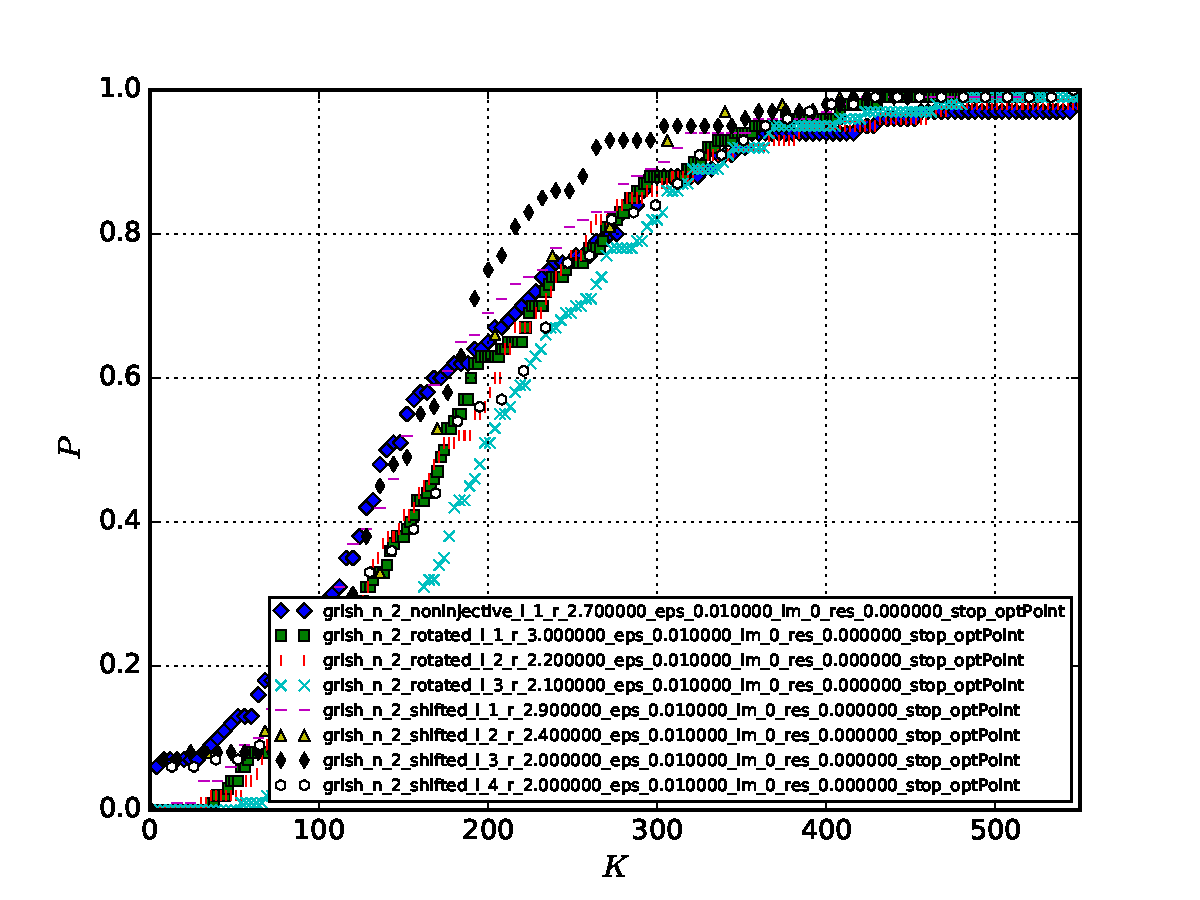
\includegraphics[width=0.95\textwidth]{../f_gr/opt_point/grish_opt_point_op.pdf}
  \caption{$F_{GR}$, остановка по попаданию в окрестность, минимальное значение $r$}
  \label{fig:}
\end{figure}

\begin{figure}[H]
  \center
  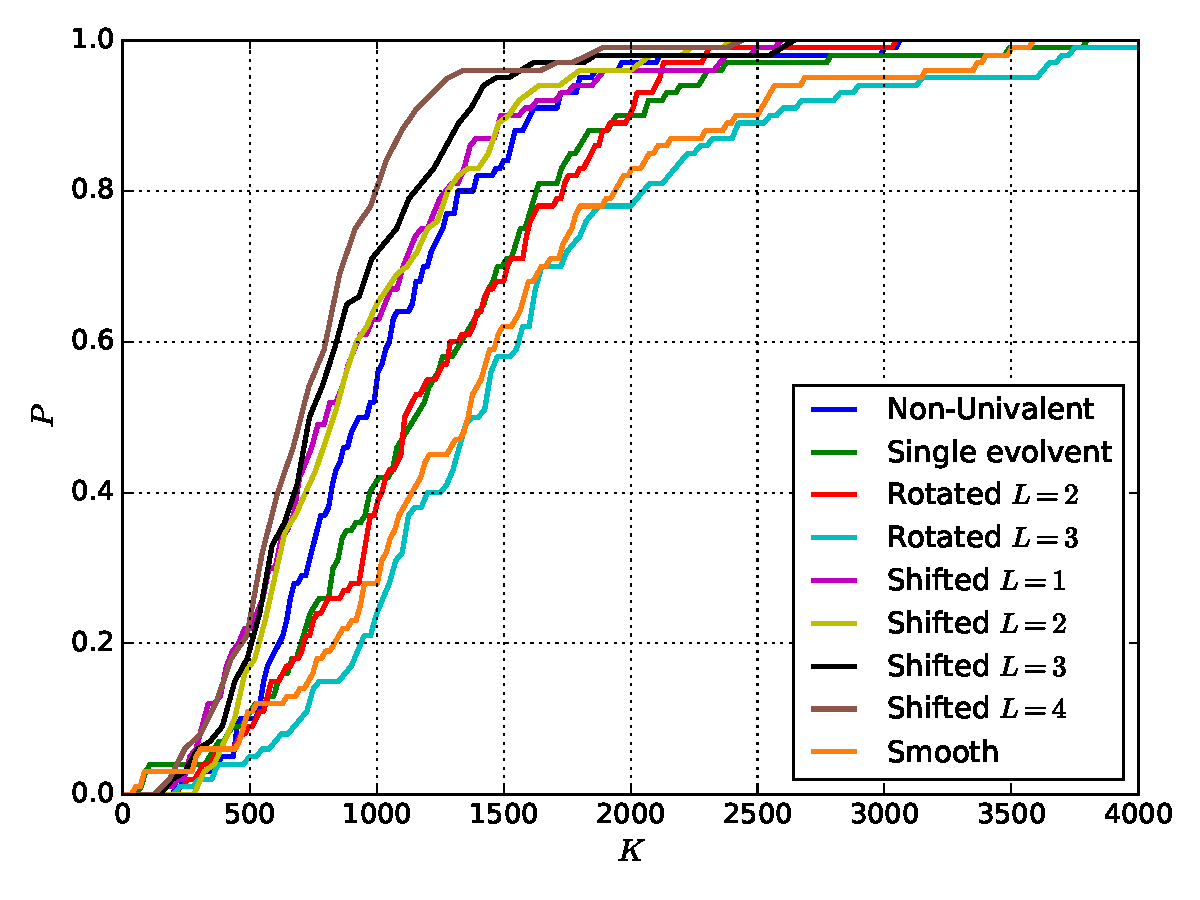
\includegraphics[width=0.95\textwidth]{../f_gr/accuracy/grish_accur_op.pdf}
  \caption{$F_{GR}$, остановка по точности, минимальное значение $r$}
  \label{fig:}
\end{figure}

\begin{figure}[H]
  \center
  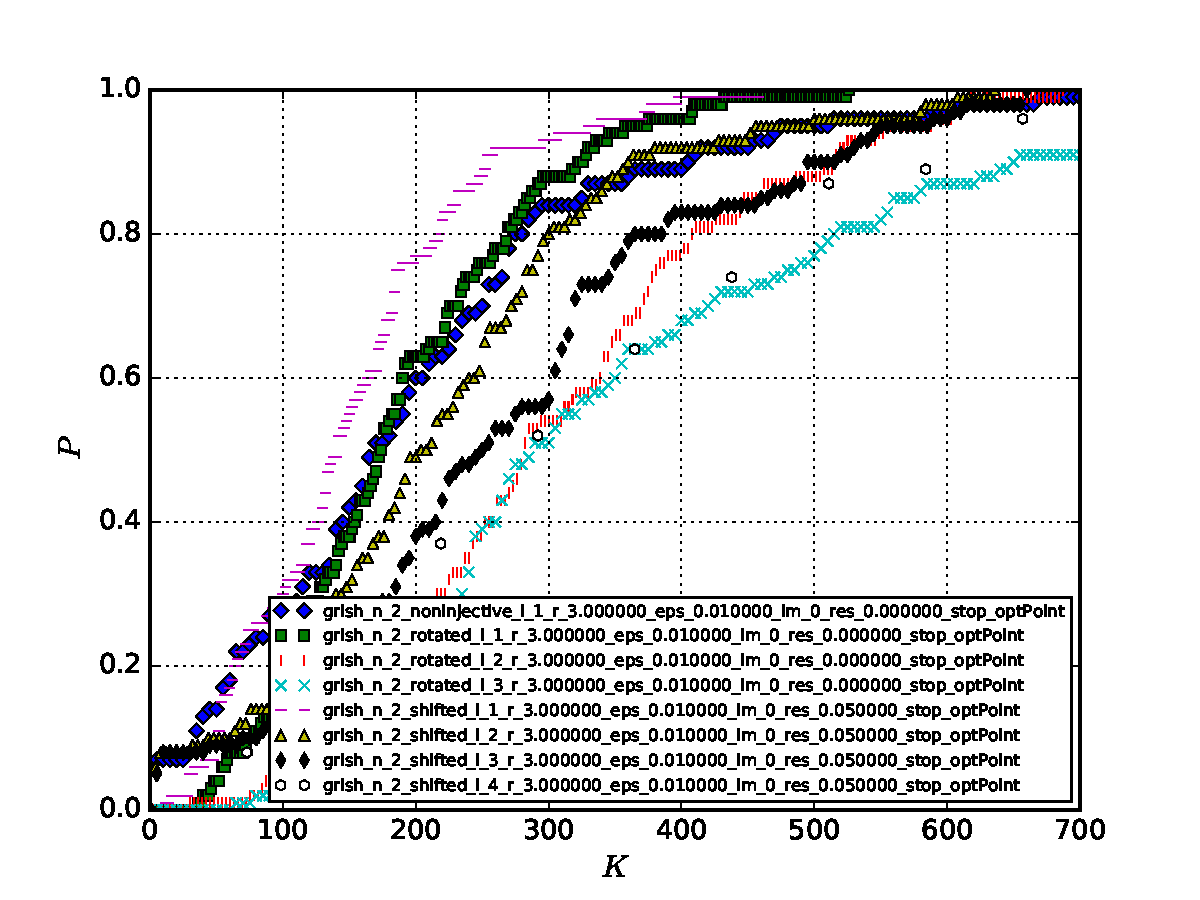
\includegraphics[width=0.95\textwidth]{../f_gr/same_r/opt_point/grish_same_r_opt_point.pdf}
  \caption{$F_{GR}$, остановка по попаданию в окрестность, $r=3.0$}
  \label{fig:}
\end{figure}

\begin{figure}[H]
  \center
  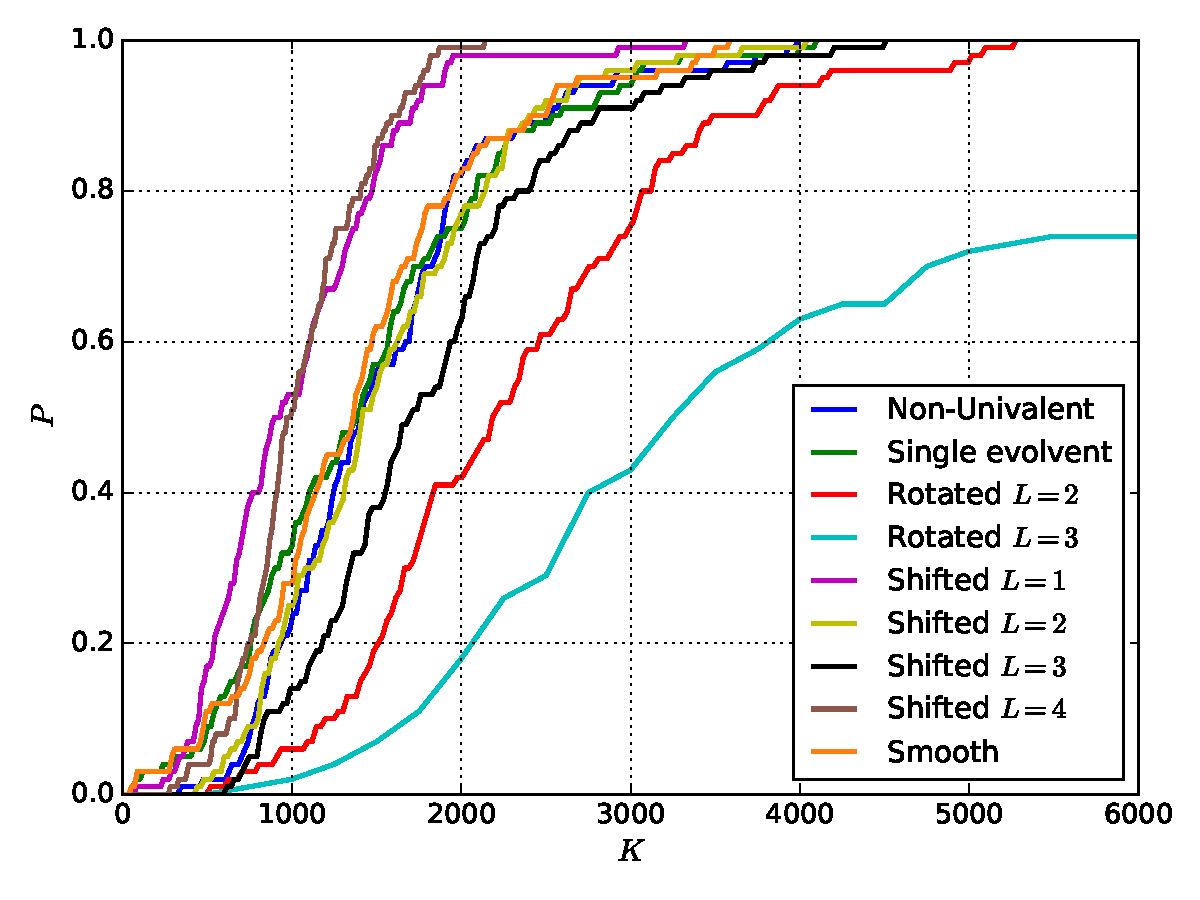
\includegraphics[width=0.95\textwidth]{../f_gr/same_r/accuracy/grish_same_r_acc.pdf}
  \caption{$F_{GR}$, остановка по точности, $r=3.1$}
  \label{fig:}
\end{figure}

\subsubsection{Класс gklsS2d}
В случае остановки по попаданию в окрестность оптимума, преимуществ от использования
множественных развёрток нет.

При остановке по точности ускорение от сдвиговой развёртки отностительно других есть
как с минимальным подобранным $r$, так и при одинаковом значении надёжности для всех
экспериментов.

Эффект ускорения при использовании одной сдвиговой развёртки так же проявляется в некоторых экспериментах.

\begin{figure}
  \center
  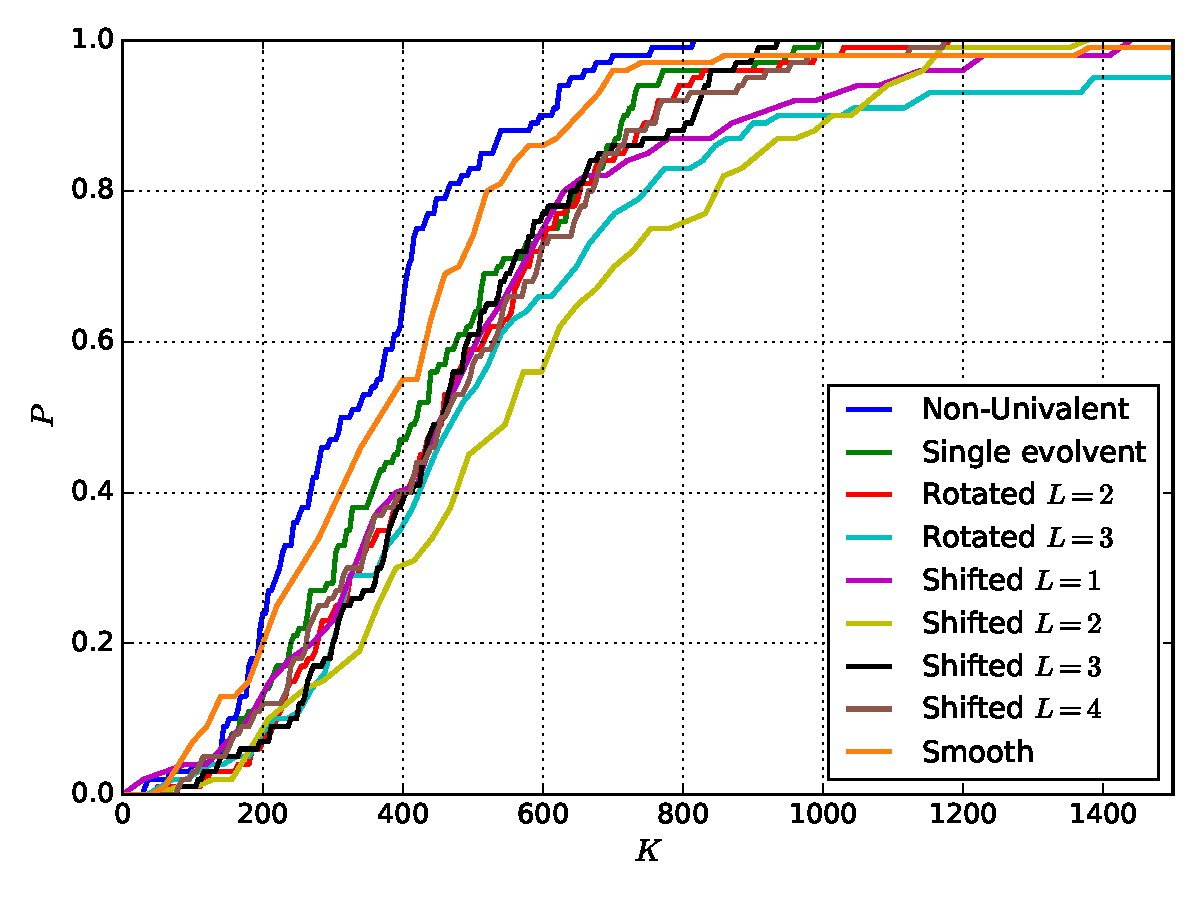
\includegraphics[width=0.95\textwidth]{../gklsS2d/opt_point/gklsS2d_opt_pt_op.pdf}
  \caption{gklsS2d, остановка по попаданию в окрестность, минимальное значение $r$}
  \label{fig:}
\end{figure}

\begin{figure}[H]
  \center
  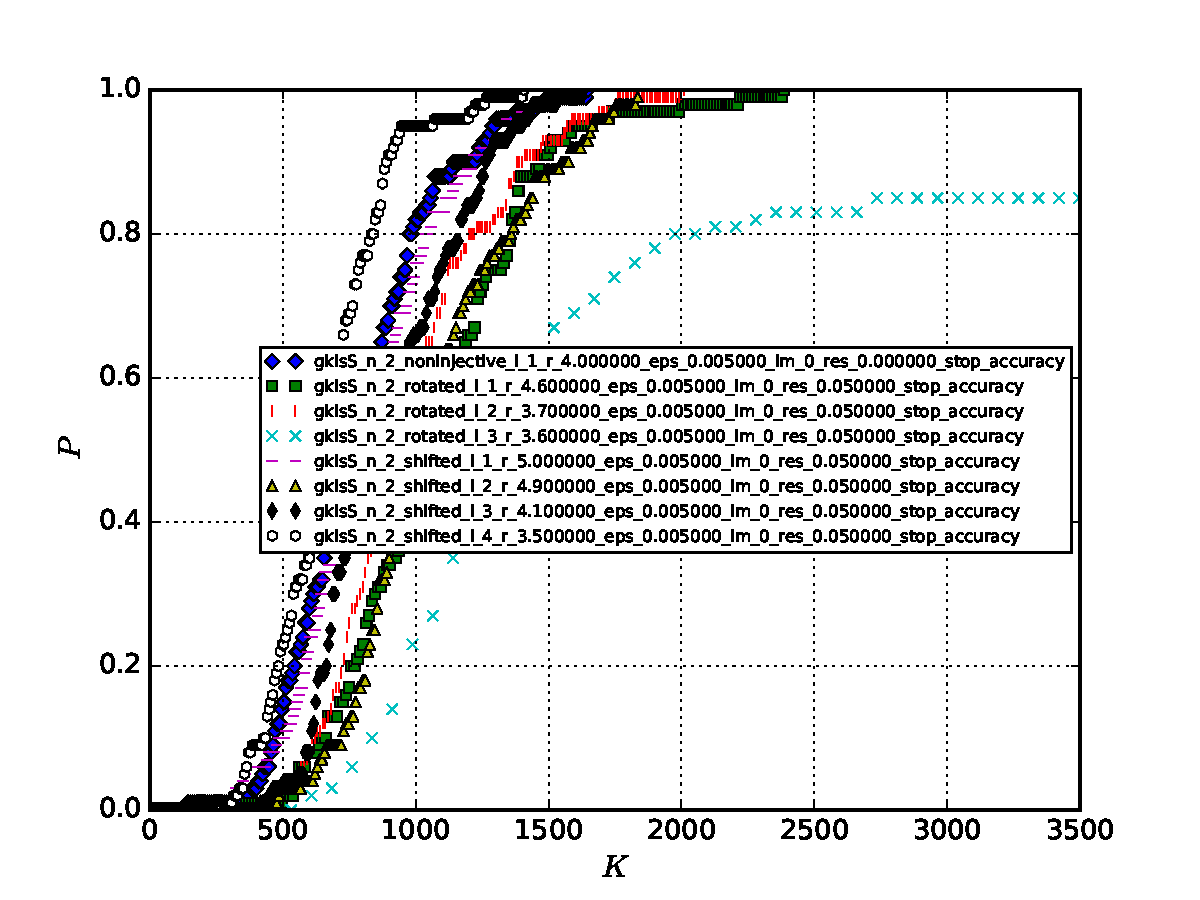
\includegraphics[width=0.95\textwidth]{../gklsS2d/accuracy/gklsS2d_acc_op.pdf}
  \caption{gklsS2d, остановка по точности, минимальное значение $r$}
  \label{fig:}
\end{figure}

\begin{figure}[H]
  \center
  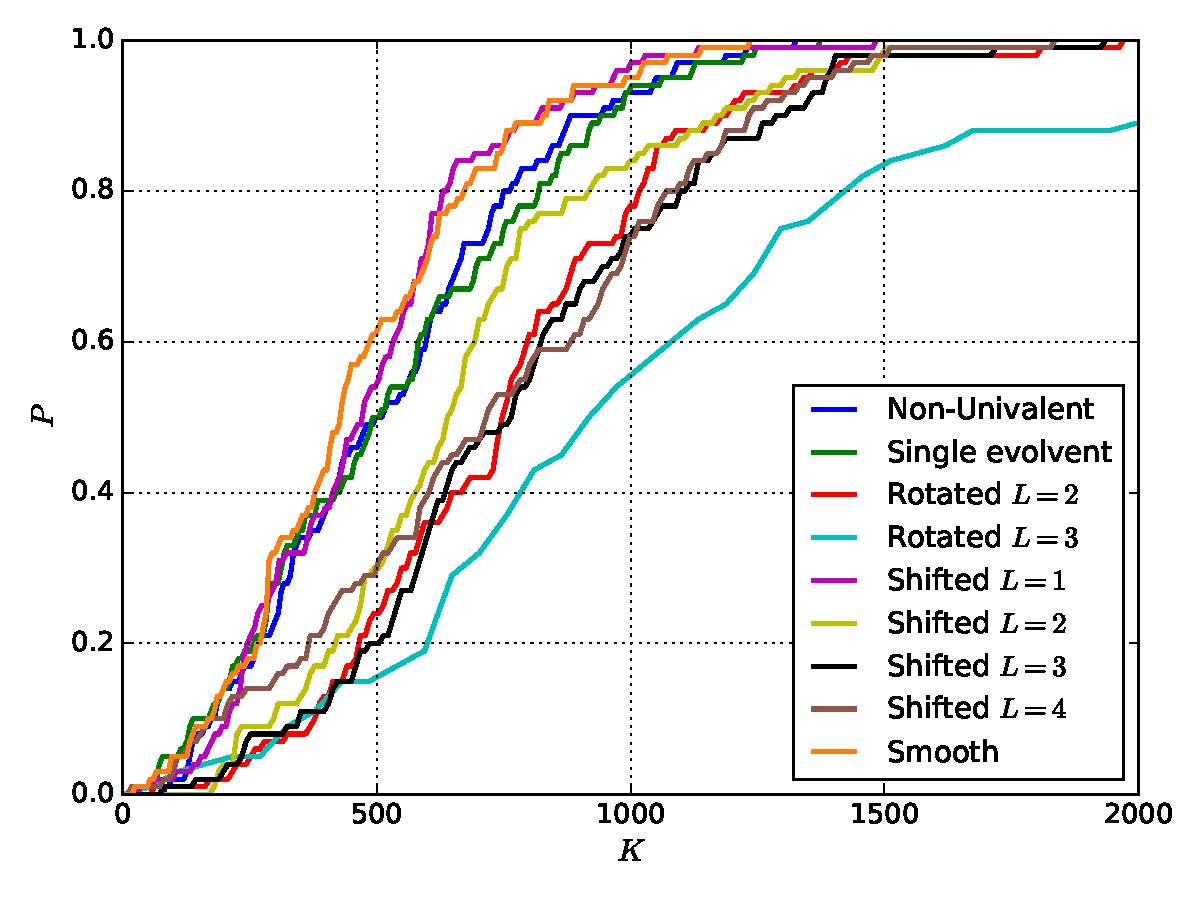
\includegraphics[width=0.95\textwidth]{../gklsS2d/same_r/opt_point/gklsS2d_same_r_opt_pt_op.pdf}
  \caption{gklsS2d, остановка по попаданию в окрестность, $r=5.0$}
  \label{fig:}
\end{figure}

\begin{figure}[H]
  \center
  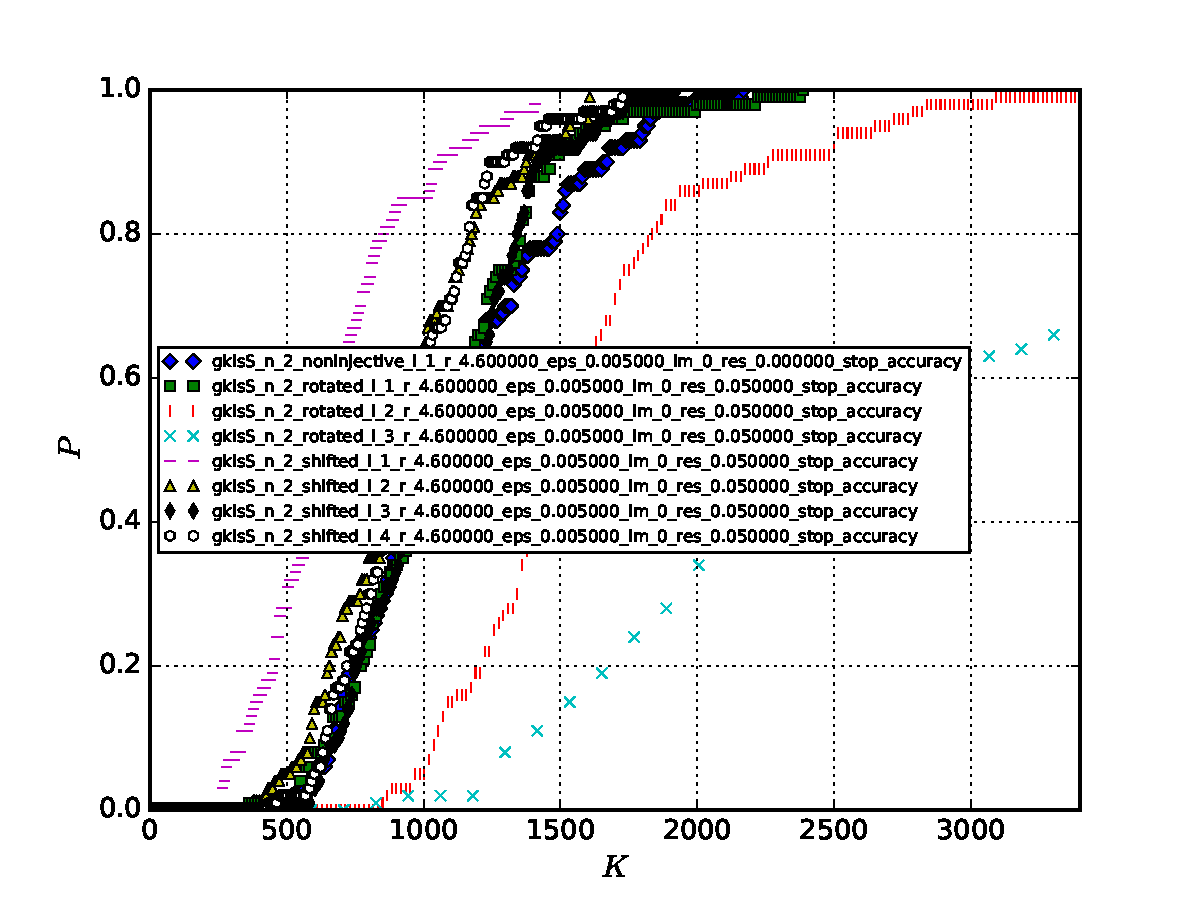
\includegraphics[width=0.95\textwidth]{../gklsS2d/same_r/accuracy/gkls2d_same_r_acc_pt_op.pdf}
  \caption{gklsS2d, остановка по точности, $r=4.6$}
  \label{fig:}
\end{figure}

\subsubsection{Класс gklsH2d}
Для этого класса удалось провести только эксперименты с одинаковым $r$ для всех вариантов метода.
Преимуществ от использования множетвенных развёрток не выявлено.

\begin{figure}
  \center
  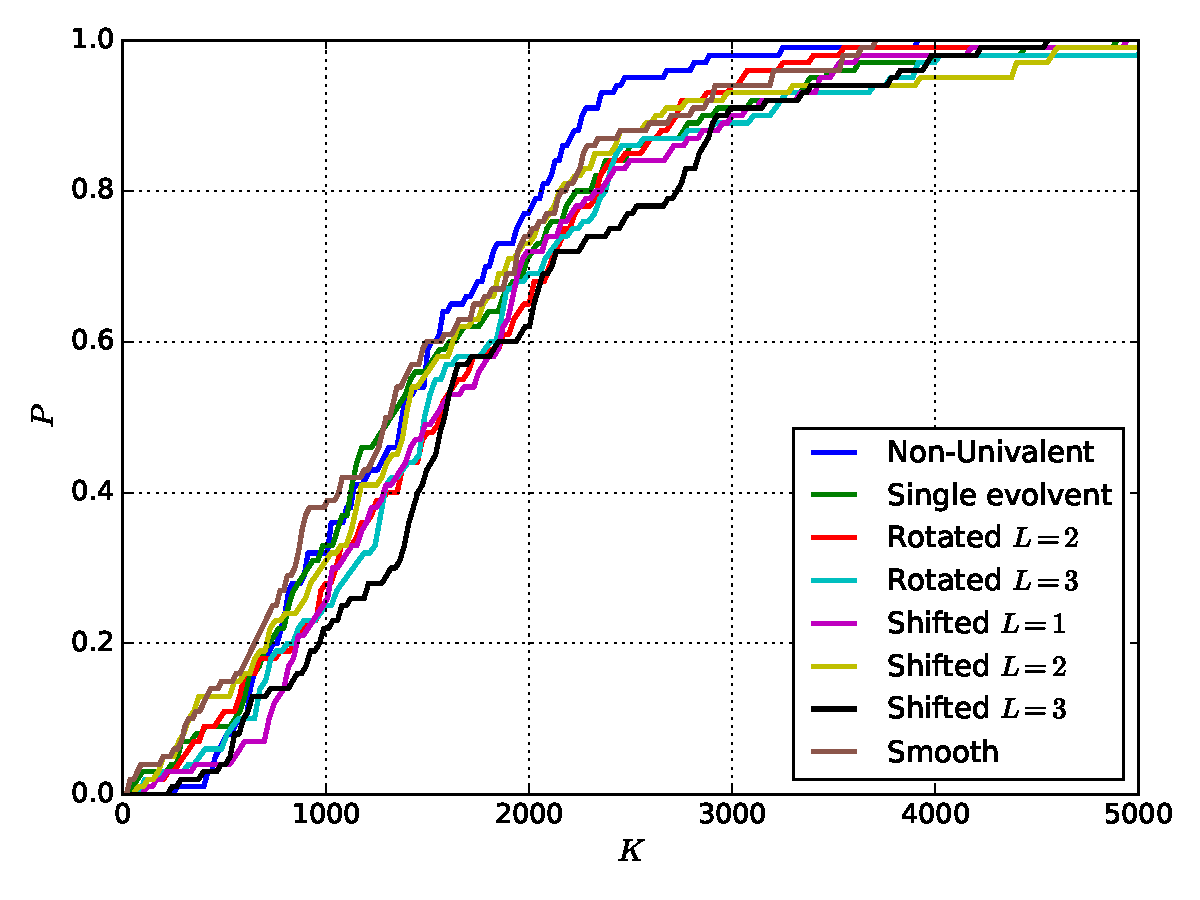
\includegraphics[width=0.95\textwidth]{../gklsH2d/opt_point/gklsH2d_opt_pt_op.pdf}
  \caption{gklsH2d, остановка по попаданию в окрестность, минимальное значение $r$}
  \label{fig:}
\end{figure}

\begin{figure}[H]
  \center
  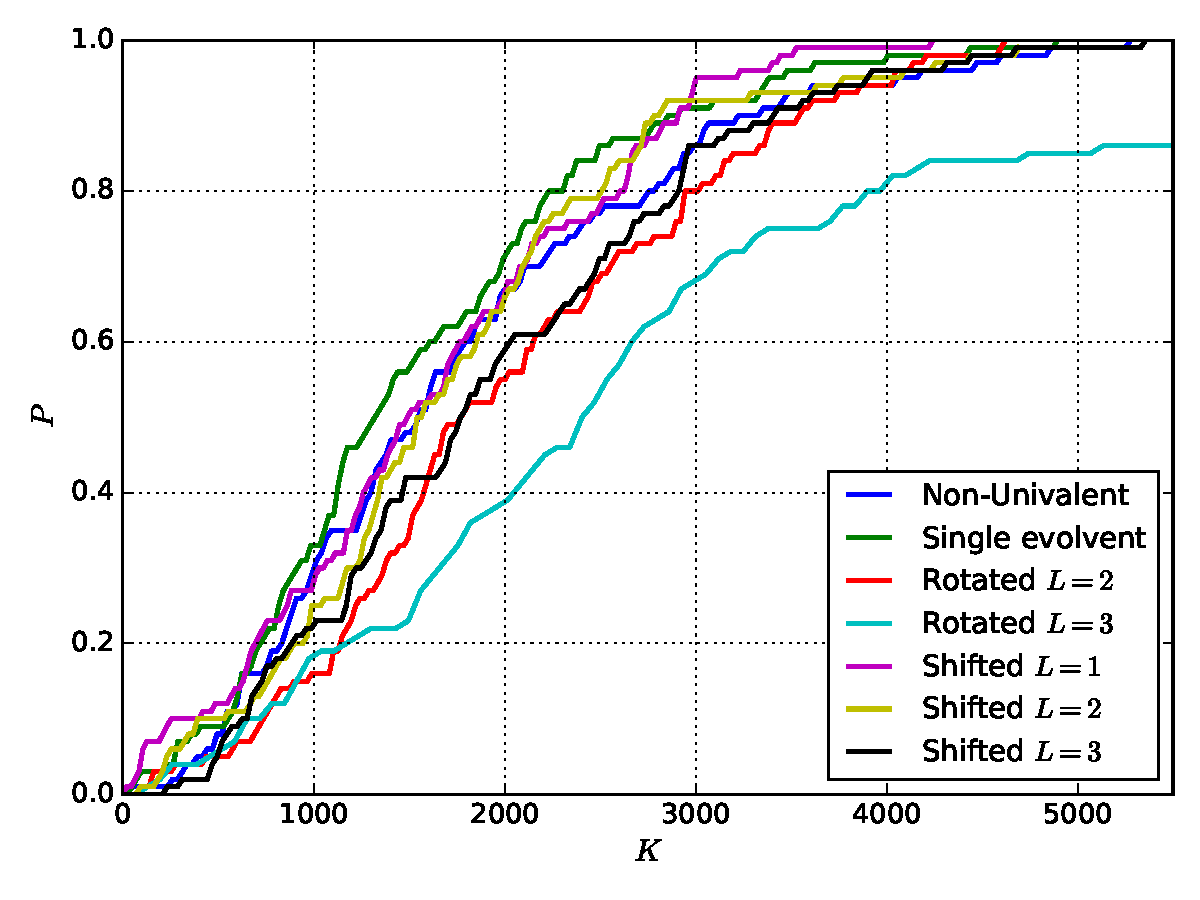
\includegraphics[width=0.95\textwidth]{../gklsH2d/same_r/opt_point/gklsH2d_same_r_opt_pt_op.pdf}
  \caption{gklsH2d, остановка по попаданию в окрестность, $r=6.6$}
  \label{fig:}
\end{figure}

\subsubsection{Класс gklsS3d}
Для этого класса удалось провести только эксперименты с одинаковым для всех вариантов метода значением $r$.
При подборе минимального $r$ сдвиговая развёртка демонстирирует преимущество.

\begin{figure}
  \center
  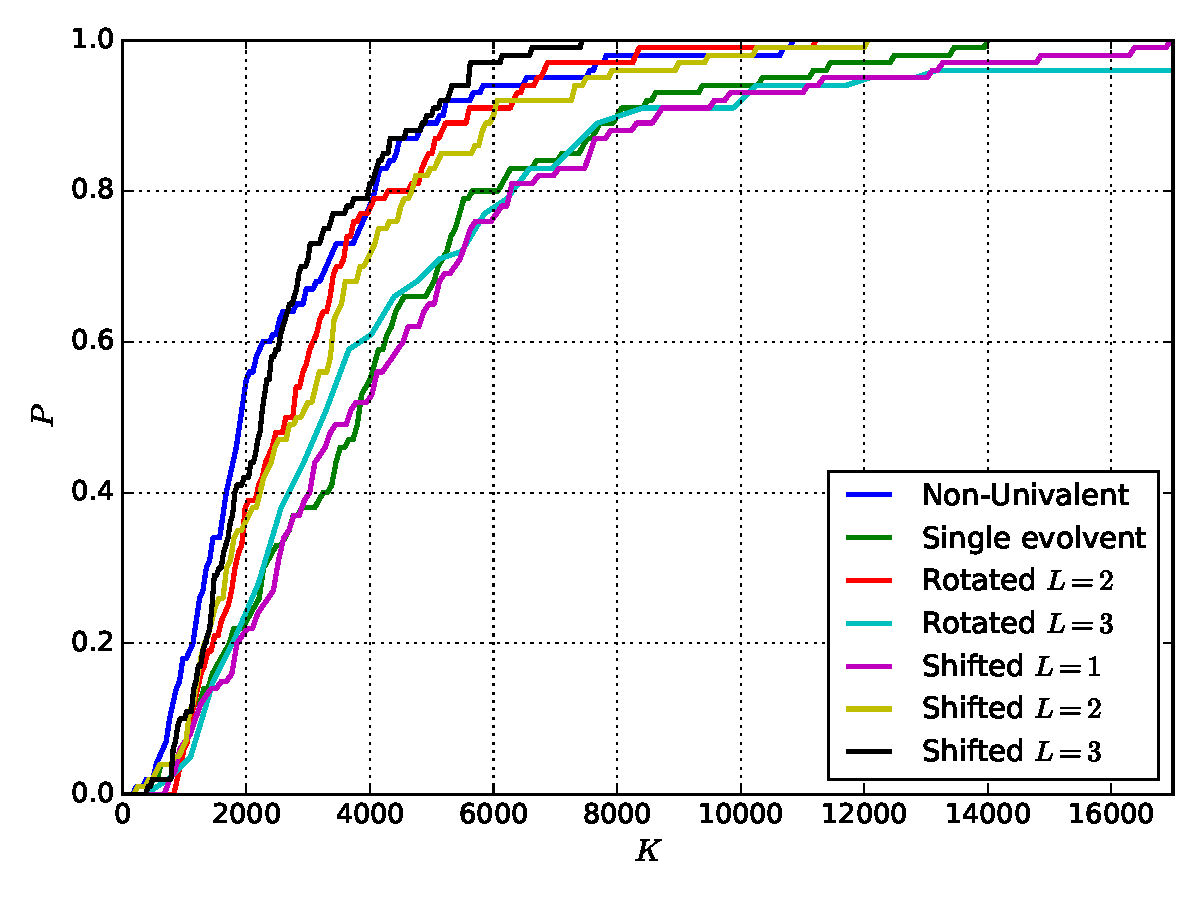
\includegraphics[width=0.95\textwidth]{../gklsS3d/opt_point/gklsS3d_opt_pt_op.pdf}
  \caption{gklsS3d, остановка по попаданию в окрестность, минимальное значение $r$}
  \label{fig:}
\end{figure}

\begin{figure}[H]
  \center
  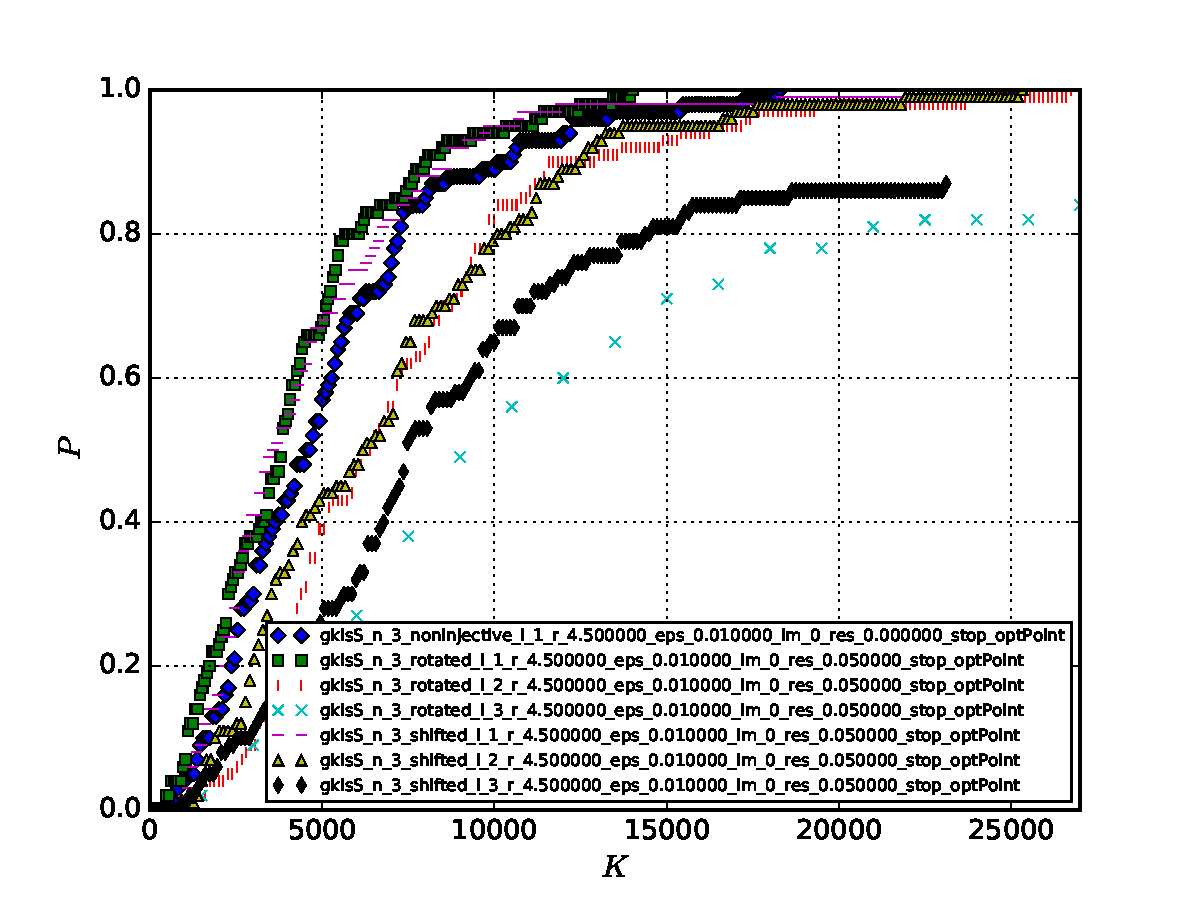
\includegraphics[width=0.95\textwidth]{../gklsS3d/same_r/opt_point/gklsS3d_same_r_opt_pt_op.pdf}
  \caption{gklsS3d, остановка по попаданию в окрестность, $r=5.0$}
  \label{fig:}
\end{figure}

\subsection{Среднее количество вычислений целевой функции}
В этом разделе приведено среднее значение количества обращений к целевой функции и к дополнительному ограничению в случае
вращаемой развёртки для каждого эксперимента. Также в каждом эксперименте вычислены отношение
количества обращений к нулевому ограничению к количеству обращений к целевой функции ($\frac{constraint}{objective}$ ratio) и
ускорение по обращениям к целевой функции от использования сдвиговой развёртки сравнению с методом с одной развёрткой ($\frac{single\_objective}{shifted\_objective}$).

\begin{table}[H]
\begin{center}
\caption{Класс $F_{GR}$, остановка по точности, минимальное значение $r$, $\varepsilon_r=0$}
  \begin{tabular}{l|l*{5}{c}}
  L & Constraint & Objective (shifted) & $\frac{constraint}{objective}$ ratio & Objective (rotated) & $\frac{single\_objective}{shifted\_objective}$ ratio \\
  \hline
  1 & 1529.98 & 941.89 & 1.64 & 1216.72 & 1.29 \\
  2 & 1835.45 & 928.93 & 1.97 & 1215.93 & 1.31 \\
  3 & 1893.67 & 840.6  & 2.25 & 1532.94 & 1.45 \\
  4 & 2690.71 & 737.18 & 3.65 &  - & 1.65 \\
  \end{tabular}
\end{center}
\end{table}

\begin{table}[H]
\begin{center}
\caption{Класс $F_{GR}$, остановка по попаданию в окрестность, минимальное значение $r$, $\varepsilon_r=0$}
  \begin{tabular}{l|l*{5}{c}}
  L & Constraint & Objective (shifted) & $\frac{constraint}{objective}$ ratio & Objective (rotated) & $\frac{single\_objective}{shifted\_objective}$ ratio \\
  \hline
  1 & 356.15 & 169.52 & 2.10 & 189.16 & 1.12 \\
  2 & 555.52 & 172.94 & 3.21 & 193.65 & 1.09 \\
  3 & 476.61 & 162.34 & 2.93 & 216.94 & 1.17 \\
  4 & 931.61 & 188.43 & 4.94 &  -     & 1.00 \\
  \end{tabular}
\end{center}
\end{table}

\begin{table}[H]
\begin{center}
\caption{Класс gklsS2d, остановка по точности, $r=4.6$, $\varepsilon_r=0.05$}
  \begin{tabular}{l|l*{5}{c}}
  L & Constraint & Objective (shifted) & $\frac{constraint}{objective}$ ratio & Objective (rotated) & $\frac{single\_objective}{shifted\_objective}$ ratio \\
  \hline
  1 & 1026.79 & 652.1   & 1.57  & 1073.25 & 1.65 \\
  2 & 2051.62 & 920.39  & 2.23  & 1579.11 & 1.17 \\
  3 & 2965.2  & 1081.43 & 2.74  & 6124.31 & 0.99 \\
  4 & 43085.8 & 952.31  & 45.24 & -       & 1.13 \\
  \end{tabular}
\end{center}
\end{table}

\begin{table}[H]
\begin{center}
\caption{Класс gklsS3d, остановка по попаданию в окрестность, минимальное значение $r$, $\varepsilon_r=0.05$}
  \begin{tabular}{l|l*{5}{c}}
  L & Constraint & Objective (shifted) & $\frac{constraint}{objective}$ ratio & Objective (rotated) & $\frac{single\_objective}{shifted\_objective}$ ratio \\
  \hline
  1 & 20570.7  & 4547.26 &  4.52 & 4231.64 & 0.93 \\
  2 & 42721.7  & 3249.85 & 13.15 & 3048.15 & 1.30 \\
  3 & 55622.7  & 2573.00 & 21.62 & 5814.08 & 1.64 \\
  \end{tabular}
\end{center}
\end{table}

\begin{table}[H]
\begin{center}
\caption{Класс gklsS3d, остановка по попаданию в окрестность, $r=5.0$, $\varepsilon_r=0.05$}
  \begin{tabular}{l|l*{5}{c}}
  L & Constraint & Objective (shifted) & $\frac{constraint}{objective}$ ratio & Objective (rotated) & $\frac{single\_objective}{shifted\_objective}$ ratio \\
  \hline
  1 & 23120.5  & 4587.49 &  5.04 & 4231.64 & 0.92 \\
  2 & 96247.9  & 6840.14 & 14.07 & 7272.07 & 0.62 \\
  3 & 153131.0 & 7702.82 & 19.88 & 26050.4 & 0.55 \\
  \end{tabular}
\end{center}
\end{table}

\section{Предварительные выводы}
\begin{itemize}
  \item Вращаемая развёртка в лучшем случае не приносит увеличения количества вычислений целевой функции по сравнению с одной развёрткой, а чаще всего оно увеличивается. Это лучше всего видно в таблицах (столбец Objective (rotated)).
  \item При использовании сдвиговой развёртки количество обращений к дополнительному ограничению может на порядок превышать количество обращений к целевой функции, а это значит, что объем поисковой информации значительно превосходит таковой при использовании сдвиговых развёрток. Это продемонстрировано в столбце $\frac{constraint}{objective}$ ratio таблиц из предыдущего раздела.
  \item Использование множественных развёрток ведёт к более качественной оценке константы Гёльдера, а значит, можно использовать меньшее значение $r$, чем для метода с одной развёрткой. Завышение $r$ чаще всего ведёт к более медленной сходимости метода с множественными развёртками, чем метода с одной развёрткой и тем же значением $r$. Это зависит от задач и критерия остановки.
  \item Сдвиговая развёртка обеспечивает преимущество над вращаемой при остановке по точности даже без подбора $r$ (но только ели задачи достаточно сложные с токи зрения метода). Если работает критерий остановки по попаданию в окрестность оптимума, то ускорения от сдвиговой развёртки обнаружено не было.
\end{itemize}




\end{document}
